\documentclass[11pt]{article}

\usepackage[a4paper,margin=1in]{geometry}
\usepackage{amsmath, amssymb, mathtools}
\usepackage{tikz}
\usetikzlibrary{calc}
\usepackage{pgfplots}
\pgfplotsset{compat=1.18}
\usetikzlibrary{positioning, arrows.meta, shapes.geometric}
\usepackage{xcolor}
\definecolor{DollarColor}{RGB}{107, 128, 104}
\definecolor{EuroColor}{RGB}{93, 126, 167}
\definecolor{BitcoinColor}{RGB}{247, 147, 26}
\usepackage{minted}
\usepackage{siunitx}
\usepackage{booktabs, array, tabularx}
\usepackage[linesnumbered,ruled,vlined]{algorithm2e}
\usepackage{hyperref}

\begin{document}

\title{Fast Arbitrage Detection}
\author{Claudio Raimondi}
\date{\today}
\maketitle

//TODO properly refer to the reader as "we" or "I". not both

\begin{abstract}
Triangular arbitrage offers opportunities to exploit price inefficiencies between three currency pairs. While several algorithms exist for triangular arbitrage detection, their computational efficiency and accuracy can vary. In this report, I present a straight forward method that combines logarithmic properties with numerical representation techniques to efficiently detect arbitrage opportunities.
\end{abstract}

\tableofcontents

\section{Introduction}
The process to exploit triangular arbitrage opportunities involves 3 generic steps, each crucial for ensuring the success of the strategy:
\begin{enumerate}
    \item \textbf{Data Collection:} Gather real-time exchange rates for the currency pairs involved.
    \item \textbf{Data Manipulation:} Use the collected data to detect profitable trades.
    \item \textbf{Execution:} Execute trades to lock in profits.
\end{enumerate}
For all three steps, the \textbf{speed} and \textbf{accuracy} of the algorithm are paramount. All the efforts become vain if somebody else collets, manipulates, and executes the arbitrage opportunity before you do.
On this report, I will focus on the \textbf{second step}---\textit{data manipulation}---, which is the most short-lived. The other two steps rely on external factors, such as networks and exchange APIs.

\section{Representation}
To visualize triangular arbitrage, we can represent it as a \textbf{directed graph} (more precisely a clique), where each node represents a currency and each edge represents an exchange rate.

\begin{center}
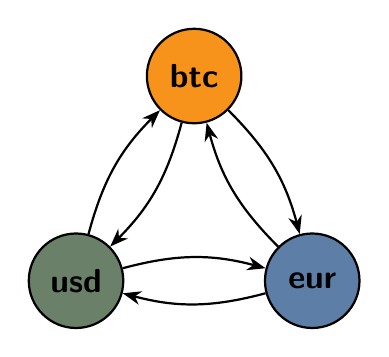
\begin{tikzpicture}[>=Stealth, thick, main/.style={draw, circle, minimum size=1.2cm, font=\sffamily\large\bfseries}]

\coordinate (A) at (0,0);
\coordinate (B) at (3,0);
\coordinate (C) at ($(A)!0.5!(B) + (0,2.6)$);

\node[main, fill=DollarColor]  (usd) at (A) {usd};
\node[main, fill=EuroColor]    (eur) at (B) {eur};
\node[main, fill=BitcoinColor] (btc) at (C) {btc};

\draw[->] (usd) to[bend left=15] node[above] {} (eur);
\draw[->] (eur) to[bend left=15] node[above] {} (btc);
\draw[->] (btc) to[bend left=15] node[above] {} (usd);

\draw[->] (eur) to[bend left=15] node[above] {} (usd);
\draw[->] (btc) to[bend left=15] node[above] {} (eur);
\draw[->] (usd) to[bend left=15] node[above] {} (btc);

\end{tikzpicture}
\end{center}

\section{Arbitrage Formula}

\subsection{Base Formula}
The formula to detect a profitable triangular arbitrage path, given three exchange rates $R$, is the following inequality:
\begin{equation}
    R_{1} \cdot R_{2} \cdot R_{3} > 1
\end{equation}

\subsection{Floating-Point Representation}
In practice, each price is a floating-point number, and often times, if the \textit{data collection} layer is serious about efficiency, they are provided as \textbf{mantissa} ($m$) and \textbf{exponent} ($e$) separately. So our inequality becomes:

\begin{equation}
    \left( m_1 \cdot 10^{e_1} \right) \cdot \left( m_2 \cdot 10^{e_2} \right) \cdot \left( m_3 \cdot 10^{e_3} \right) > 1
\end{equation}
\begin{equation}
    m_1 \cdot m_2 \cdot m_3 \cdot 10^{e_1 + e_2 + e_3} > 1
\end{equation}
\begin{equation}
    m_1 \cdot m_2 \cdot m_3 > \frac{1}{10^{e_1 + e_2 + e_3}}
\end{equation}
\begin{equation}
    m_1 \cdot m_2 \cdot m_3 > 10^{-(e_1 + e_2 + e_3)}
\end{equation}

\subsection{Logarithmic Form}
In most computer systems, where registers are limited to 64 bits, the product of three mantissas can easily overflow. To address this, we can use logarithmic properties to transform the \textbf{product} into an \textbf{addition} of much smaller numbers and the \textbf{power} into a \textbf{product}:
\begin{equation}
    \log_b(m_1 \cdot m_2 \cdot m_3) > \log_b(10^{-(e_1 + e_2 + e_3)})
\end{equation}
\begin{equation}
    \log_b(m_1) + \log_b(m_2) + \log_b(m_3) > -(e_1 + e_2 + e_3) \cdot \log_b(10)
\end{equation}

\subsection{Inverse Direction}
As of now, we have only considered the \textbf{forward direction} of the triangular arbitrage, i.e. the forward cycle path. But since the rates are bidirectional, we can also exploit price inefficiencies in the \textbf{reverse direction}. Assuming we don't have the rates for the reverse direction, we can compute them as the inverse of the forward rates, and the formula becomes:
\setcounter{equation}{0}
\begin{equation}
    \frac{1}{R_{1}} \cdot \frac{1}{R_{2}} \cdot \frac{1}{R_{3}} > 1
\end{equation}
\begin{equation}
    \frac{1}{m_1 \cdot 10^{e_1}} \cdot \frac{1}{m_2 \cdot 10^{e_2}} \cdot \frac{1}{m_3 \cdot 10^{e_3}} > 1
\end{equation}
\begin{equation}
    \frac{1}{m_1 \cdot m_2 \cdot m_3 \cdot 10^{e_1 + e_2 + e_3}} > 1
\end{equation}
\begin{equation}
    m_1 \cdot m_2 \cdot m_3 \cdot 10^{e_1 + e_2 + e_3} < 1
\end{equation}
\begin{equation}
    m_1 \cdot m_2 \cdot m_3 < \frac{1}{10^{e_1 + e_2 + e_3}}
\end{equation}
\begin{equation}
    m_1 \cdot m_2 \cdot m_3 < 10^{-(e_1 + e_2 + e_3)}
\end{equation}
\begin{equation}
    \log_b(m_1 \cdot m_2 \cdot m_3) < \log_b(10^{-(e_1 + e_2 + e_3)})
\end{equation}
\begin{equation}
    \log_b(m_1) + \log_b(m_2) + \log_b(m_3) < -(e_1 + e_2 + e_3) \cdot \log_b(10)
\end{equation}

\section{Algorithm}

\subsection{The Spread Problem}
Once the formula is derived, the algorithm is just a matter of applying the two inequalities. From a first analysis, it seems that the only difference between the forward and reverse inequalities is their direction. However, we have to account for the \textbf{spread}, which is the difference between the bid and ask prices. This means that we have to consider the \textbf{ask} price for the forward direction and the \textbf{bid} price for the reverse direction.

\subsection{The choice of the base}
Up to this point, we have considered the base $b$ of the logarithm to be arbitrary. But in practice, we have to choose the one that best fits our needs.
\begin{itemize}
    \item $\log_{2}$ matches the binary representation of floating-point numbers.
    \item $\log_{10}$ allows for a simplification of the formula: $\log_{10}(10) = 1$.
\end{itemize}
In this implementation, we choose $\log_{2}$. This decision is motivated by \textbf{efficiency} and \textbf{precision}. In fact, since floating-point numbers are naturally represented in base 2, we can compute the logarithm with fast bit-shifts and with zero precision loss. Additionally, the simplification of the formula that comes with $\log_{10}$ is not necessary, as we can precompute it.

\subsection{Precomputation}
Assuming exponents change very rarely, we can use an optimistic approach and \textbf{precompute} the entire right side of the inequality, storing it in a constant variable, raising an exception or even updating the precomputed constant only when the exponents change.

\subsection{The Representation of real numbers}
The logarithms produce real numbers. To address this in an effient manner, we must avoid floating-point numbers once again. This leaves us with two options:
\begin{enumerate}
  \item \texttt{log2(integer x) $\rightarrow$ FixedPoint}
  \item \texttt{log2(integer x) $\rightarrow$ [Mantissa, Exponent]}
\end{enumerate}
While both are great alternatives, the latter is preferable because we can choose the base of the returned floating-point representation. Furthermore, if we choose the same base as the logarithm, there is a lot of room for optimization.

\subsection{The Actual Computation}
Combining all the previous steps, we can derive the final steps to compute the left side of the inequality:
\setcounter{equation}{0}
\begin{equation}
    \log_2(m_1) + \log_2(m_2) + \log_2(m_3)
\end{equation}
\begin{equation}
    m'_1 \cdot 2^{e'_1} + m'_2 \cdot 2^{e'_2} + m'_3 \cdot 2^{e'_3}
\end{equation}
computing the maximum exponent $e'_{\max}$ for normalization:
\begin{equation}
    (m'_1 \cdot 2^{e'_1 - e'_{\max}}) \cdot 2^{e'_{\max}} + (m'_2 \cdot 2^{e'_2 - e'_{\max}}) \cdot 2^{e'_{\max}} + (m'_3 \cdot 2^{e'_3 - e'_{\max}}) \cdot 2^{e'_{\max}}
\end{equation} 
\begin{equation}
    2^{e'_{\max}} \cdot (m'_1 \cdot 2^{e'_1 - e'_{\max}} + m'_2 \cdot 2^{e'_2 - e'_{\max}} + m'_3 \cdot 2^{e'_3 - e'_{\max}})
\end{equation}
rewriting the powers of two as bitshifts:
\begin{equation}
    (m'_1 \ll (e'_1 - e'_{\max}) + m'_2 \ll (e'_2 - e'_{\max}) + m'_3 \ll (e'_3 - e'_{\max})) \ll e'_{\max}
\end{equation}


\subsection{Log2}
//TODO actual log2 implementation

\begin{minted}{c}
void normalize(uint64_t value, uint64_t &mantissa, uint8_t &exponent)
{
  uint8_t leading_zeros = __builtin_clzll(value);
  exponent = 63 - leading_zeros;
  mantissa = value << leading_zeros;
}
\end{minted}

\section{Bellman-Ford Algorithm}

\section{Relative Error}

\section{Optimization}
% parallelization (either of the bellman-ford or of the 2 formulas (6 logs in parallel))

\begin{thebibliography}{9}


\end{thebibliography}

\end{document}
